\section{Method}
\label{sec:method}

\subsection{Preliminaries}

The goal of reinforcement learning is to learn a policy that maximizes the expected cumulative discounted reward in a Markov decision process (MDP) \cite{sutton1999reinforcement} defined by the tuple $(\mathcal{S}, \mathcal{A}, P, R, \gamma)$, where $\mathcal{S}$ is the state space, $\mathcal{A}$ is the action space, $P(s'|s, a)$ is the transition probability, $R(s, a)$ is the reward function, and $\gamma \in (0, 1)$ is the discount factor. The agent interacts with the environment by following a policy $\pi(a|s)$, which maps states to actions. The state value function $V^{\pi}(s)$ and the action-value function $Q^{\pi}(s, a)$ are defined as the expected cumulative discounted reward under policy $\pi$ starting from state $s$ and taking action $a$. The optimal value functions $V^*(s)$ and $Q^*(s, a)$ are defined as the maximum value functions over all policies, which satisfy the Bellman equation
\begin{equation}
    \begin{aligned}
        V^*(s) &= \max_{\pi} \mathbb{E}_{a \sim \pi(\cdot|s)} \left[ Q^{\pi}(s, a) \right] \\
        Q^*(s, a) &= R(s, a) + \gamma \mathbb{E}_{s' \sim P(\cdot|s, a)} \left[ \max_{a'} Q^*(s', a') \right]
    \end{aligned}
\end{equation}
In the offline setting, the environment is not accessible when training, so the agent can only learn from a fixed dataset $\mathcal{D} = \{(s_i, a_i, r_i, s'_i)\}_{i=1}^N$ collected by a behavior policy $\pi_{\beta}(a|s)$, where $s_i$ is the state, $a_i$ is the action, $r_i$ is the reward, $s'_i$ is the next state, and $N$ is the number of transitions. In the multi-task setting, the dataset $\mathcal{D}=\cup_{i=1}^M \mathcal{D}_i$ consists of transitions from multiple tasks, where $\mathcal{D}_i$ is the dataset of task $i$ and $M$ is the number of tasks. The goal is to learn a policy that maximizes the expected cumulative discounted reward across all the tasks.

\subsection{Soft Actor-Critic}

Soft actor-critic (SAC) is an actor-critic algorithm that maximizes the entropy-regularized expected cumulative discounted reward \cite{haarnoja2018soft}. Different from the traditional actor-critic algorithms such as trust region policy optimization (TRPO) \cite{schulman2015trust} and proximal policy optimization (PPO) \cite{schulman2017proximal}, SAC follows an off-policy learning paradigm, which significantly improves the sample efficiency and can be better applied to the offline setting. Besides the cumulative reward, SAC also tries to maximize the entropy of the policy, which encourages exploration and prevents premature convergence to suboptimal policies. The objective function of SAC can be specified as
\begin{equation}
    J(\pi) = \sum \nolimits_{t=0}^{\infty} \mathbb{E}_{(s_t, a_t) \sim \rho_{\pi}} \left[ R(s_t, a_t) + \alpha \mathcal{H}(\pi(\cdot|s_t)) \right]
\end{equation}
where $\rho_{\pi}$ is the state-action visitation distribution induced by the policy $\pi$, $\mathcal{H}(\pi(\cdot|s_t))$ is the entropy of the policy, and $\alpha$ is the temperature parameter that determines the relative importance of the entropy term. Then the policy evaluation step should be modified to match the entropy-regularized objective. The soft Q-value can be computed by iteratively applying a modified Bellman operator
\begin{equation}
    \mathcal{T}^{\pi}Q(s, a) = R(s, a) + \gamma \mathbb{E}_{s' \sim P(\cdot|s, a)} \left[ \mathbb{E}_{a' \sim \pi(\cdot|s')} \left[ Q(s', a') - \alpha \log \pi(a'|s') \right] \right]
\end{equation}
Theoretical analysis shows that the soft Q-value will finally converge with enough iterations. At the same time, the policy improvement step should also be modified. SAC assumes that the policy distribution is proportional to the exponential of the soft Q-value, so the policy can be updated by minimizing the Kulback-Leibler (KL) divergence between the current policy and the normalized exponential of the soft Q-value, which can be formulated as
\begin{equation}
    \pi'(\cdot|s) = \arg \min_{\mu} D_{\text{KL}} \left( \mu(\cdot|s) \left\| \frac{\exp(Q^{\pi}(s, \cdot))}{Z^{\pi}(s)} \right. \right)
\end{equation}
where $Z^{\pi}(s)$ is the partition function that normalizes the exponential of the soft Q-value. Theoretical analysis shows that the policy is guaranteed to improve, so it will converge to the optimal policy.

In the actual implementation, several tricks are introduced to realize the expected algorithm. Firstly, SAC uses a Gaussian policy parameterized by a mean and a standard deviation, so the reparameterization trick is required to back propagate the gradient correctly. Secondly, SAC uses two Q-networks to estimate the soft Q-value and takes the minimum of the two results to avoid the overestimation of the Q-value. SAC also introduces two target Q-networks as in deep deterministic policy gradient (DDPG) \cite{lillicrap2015continuous} to update the Q-networks softly and stabilize the training process. Finally, we introduce automating entropy adjustment for maximum entropy \cite{haarnoja2018application} to adaptively choose the temperature parameter $\alpha$ during training. To be specific, it converts the entropy regularization term into a constraint and tries to solve the following constrained optimization problem
\begin{equation}
    \begin{aligned}
        \max_{\pi} & \sum \nolimits_{t=0}^{\infty} \mathbb{E}_{(s_t, a_t) \sim \rho_{\pi}} \left[ R(s_t, a_t) \right] \\
        \text{s.t. } & \mathbb{E}_{(s_t, a_t) \sim \rho_{\pi}} \left[ -\log \pi(a_t|s_t) \right] \geq \mathcal{H}_0, \forall t
    \end{aligned}
\end{equation}
where $\mathcal{H}$ is the target entropy. This constrained optimization problem can be converted into its dual form and solved by the Lagrange multiplier method. The result can be formulated as
\begin{equation}
    \alpha_t^* = \arg \min_{a_t} \mathbb{E}_{a_ t\sim \pi(\cdot|s_t)} \left[ - \alpha_t \log \pi(a_t|s_t) - \alpha_t \mathcal{H}_0 \right]
\end{equation}
where $\bar{\mathcal{H}}$ is a predefined minimum policy entropy threshold, which is empirically set to the negative of the action space dimension. Now the temperature parameter $\alpha$ can be automatically adjusted during the training process by gradient descent method. This trick is proved to be quite effective in practice and has been widely used in the SAC algorithm.

\subsection{Conservative Q-Learning}

Although researchers have proposed many methods for offline reinforcement learning, conservative Q-learning (CQL) \cite{kumar2020conservative} is still the most stable and effective method in practice. The key idea of CQL is to discourage the out-of-distribution Q-values while encouraging the Q-values in the dataset, so that the overestimation of the Q-values can be suppressed to some extent. The original form of CQL can be formulated as a family of optimization problems
\begin{equation}
    \begin{aligned}
        \min_Q \max_{\mu} &\ \alpha \left( \mathbb{E}_{s \sim \mathcal{D}, a \sim \mu(\cdot|s)} \left[ Q(s, a) \right] - \mathbb{E}_{s \sim \mathcal{D}, a \sim \pi_{\beta}(\cdot|s)} \left[ Q(s, a) \right] \right) \\
        &+ \frac{1}{2} \mathbb{E}_{(s,a,s') \sim \mathcal{D}} \left[ \left( Q(s, a) - \mathcal{B}^{\pi_k} Q^k(s, a) \right)^2 \right] + \mathcal{R}(\mu)
    \end{aligned}
\end{equation}
where $\alpha$ is the temperature parameter that determines the relative importance of the conservative term, $\mathcal{B}^{\pi_k}$ is the Bellman operator under the behavior policy $\pi_k$, and $\mathcal{R}(\mu)$ is a general regularizer. If we choose $\mathcal{R}(\mu)$ to be the KL divergence between the current policy and the uniform distribution, the optimization problem can be rearranged into the following form
\begin{equation}
    \begin{aligned}
        \min_Q &\ \alpha \mathbb{E}_{s \sim \mathcal{D}} \left[ \log \sum \nolimits_a \exp(Q(s, a)) - \mathbb{E}_{a \sim \pi_{\beta}(\cdot|s)} \left[ Q(s, a) \right] \right] \\
        &+ \frac{1}{2} \mathbb{E}_{(s,a,s') \sim \mathcal{D}} \left[ \left( Q(s, a) - \mathcal{B}^{\pi_k} Q^k(s, a) \right)^2 \right]
    \end{aligned}
\end{equation}
In continuous action spaces, the log-sum-exp operation should be approximated by importance sampling, where we can rewrite the term as
\begin{equation}
    \begin{aligned}
        \log \sum \nolimits_a \exp(Q(s, a)) &= \log \left( \frac{1}{2} \sum \nolimits_a \exp(Q(s, a)) + \frac{1}{2} \sum \nolimits_a \exp(Q(s, a)) \right) \\
        &= \log \left( \frac{1}{2} \mathbb{E}_{a\sim U(\mathcal{A})} \left[ \frac{\exp(Q(s, a))}{U(a)} \right] + \frac{1}{2} \mathbb{E}_{a\sim \pi(\cdot|s)} \left[ \frac{\exp(Q(s, a))}{\pi(a|s)} \right] \right)
    \end{aligned}
\end{equation}
where $U(\mathcal{A})$ is the uniform distribution over the action space. Then we can sample $N$ actions each from the uniform distribution and the policy distribution to effectively estimate this term. Note that CQL only makes some modifications to the objective function of the Q-network, so it can be easily combined with other actor-critic algorithms. In practice, CQL is usually combined with SAC to solve the offline reinforcement learning problems with continuous action spaces.

\subsection{Task Embedding}

Since we expect the agent to learn multiple tasks simultaneously, we need a machanism to explicitly inform the agent of which task it is currently facing. The simplest way is to separately train a policy for each task, but this method is not efficient enough and cannot fully exploit the shared representations among tasks. Scaled Q-learning \cite{kumar2022offline} uses multiple policy heads for each task which share the same backbone as the feature extractor, so that the agent can benefit from the shared feature representations across tasks. Conservative data sharing \cite{yu2021conservative} appends a one-hot vector to the state space to indicate the task, so that the agent can distinguish the tasks and learn specific policies.

Inspired by the embeddings used in transformers, we propose a similar method to specify the task information. As shown in Figure \ref{fig:task_embedding}, we assign a unique identity $k$ to each task. The identity will be fed into an embedding layer to generate the task embedding $e$, which will be added onto the state $s$ as the task-aware state $z$. The task-aware state $z$ will be fed together with the action $a$ into the critic network to output the estimated Q-value $\hat{q}$. It will also be fed alone into the actor network to output the predicted action $\hat{a}$. Note that the task embedding $e$ can be learned during the training process, which ensures that the performance of the agent will not degrade in the multi-task setting.

\begin{figure}[ht]
    \centering
    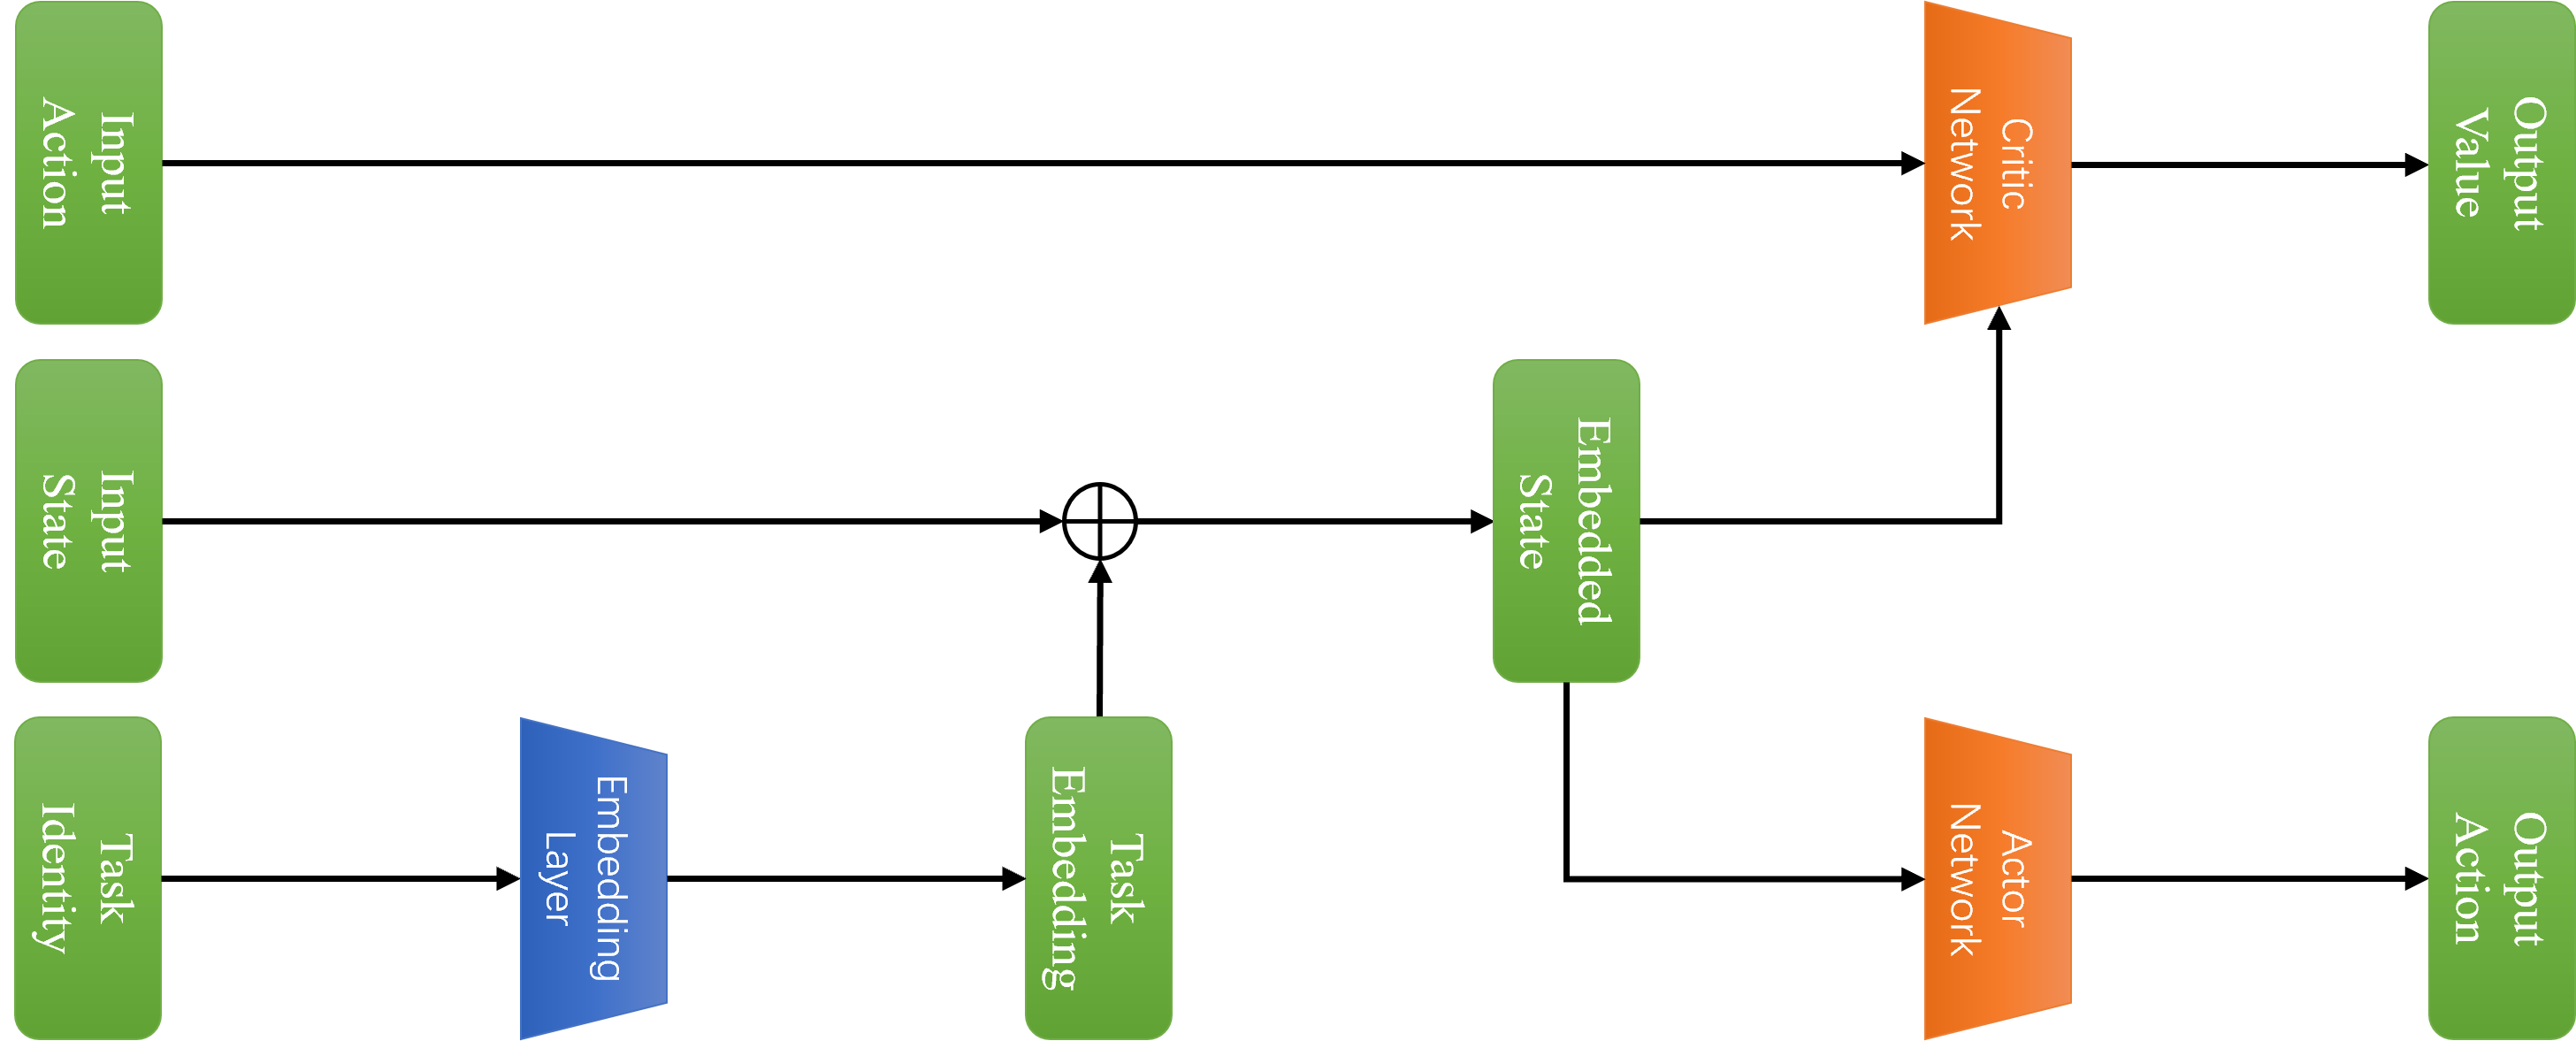
\includegraphics[width=0.8\textwidth]{figure/task_embedding.png}
    \caption{An illustration of the task embedding. The task identity $k$ is fed into an embedding layer to generate the task embedding $e$, which will be added onto the state $s$ as the task-aware state $z$. The task-aware state $z$ will be fed together with the action $a$ into the critic network to output the estimated Q-value $\hat{q}$. It will also be fed alone into the actor network to output the predicted action $\hat{a}$.}
    \label{fig:task_embedding}
\end{figure}

\subsection{Heuristic Relabeling}

Previous works \cite{yu2021conservative} have verified that one of the main reason for the failure in the multi-task setting is distribution shifts. If the agent utilizes the transitions from all the tasks without making any distinction, those out-of-distribution transitions will significantly hinder the learning process. Inspired by the idea of conservative data sharing \cite{yu2021conservative}, one feasible solution is to share the transitions conservatively. Luckily, conservative Q-learning has already provided the conservative Q-values as an indicator to measure the distribution shifts, so we define the relabeling threshold $\tau(\mathcal{D}_i)$ as
\begin{equation}
    \tau(\mathcal{D}_i) = \left\{ Q_i(s, a) | (s, a) \in \mathcal{D}_i \right\}_{k\%}
\end{equation}
where $Q_i(s, a)$ is the Q-value of the transition $(s, a)$ under the policy of task $i$, and $\{ \cdot \}_{k\%}$ denotes the $k\%$ quantile of the set. Then for any transition $(s, a, r, s') \in \mathcal{D}_j$, we can relabel $j$ as $i$ only if the conservative Q-value of the transition $(s, a)$ under the policy of task $i$ is no smaller than the relabeling threshold of $\mathcal{D}_i$, which can be formulated as
\begin{equation}
    \Delta (s, a) = Q_i(s, a) - \tau(\mathcal{D}_i) \geq 0
\end{equation}
Then we can extend the dataset $\mathcal{D}$ by adding the transitions that satisfy the relabeling condition, which can benefit the learning process of the agent. Note that the Q-network is changing during the training process, so we only relabel the dataset once in a while to ensure the stability of training. The overall pipeline of the heuristic relabeling algorithm is summarized in Algorithm \ref{alg:heuristic_relabeling}.

\begin{algorithm}[H]
    \caption{Heuristic Relabeling}
    \label{alg:heuristic_relabeling}
    \begin{algorithmic}[1]
        \REQUIRE The multi-task offline dataset $\mathcal{D}=\cup_{i=1}^M \mathcal{D}_i$.
        \STATE Initialize the active dataset $\mathcal{D}^* \leftarrow \mathcal{D}$.
        \FOR{$k \leftarrow 1, 2, \cdots, L$}
            \STATE Train the agent using samples from $\mathcal{D}^*$ to obtain the latest critic network $Q$.
            \FOR{$i \leftarrow 1, 2, \cdots, M$}
                \STATE Initialize the active dataset $\mathcal{D}_i^* \leftarrow \mathcal{D}_i$.
                \STATE Compute the relabeling threshold $\tau(\mathcal{D}_i) \leftarrow \left\{ Q(s, a) | (s, a) \in \mathcal{D}_i \right\}_{k\%}$.
                \FOR{$j \leftarrow 1, 2, \cdots, M$ where $j \neq i$}
                    \STATE Extend dataset by relabeling $\mathcal{D}_i^* \leftarrow \mathcal{D}_i^* \cup \{(s, a, r, s') \in \mathcal{D}_j | Q_i(s, a) \geq \tau(\mathcal{D}_i)\}$.
                \ENDFOR
            \ENDFOR
            \STATE Merge the active dataset $\mathcal{D}^* \leftarrow \cup_{i=1}^M \mathcal{D}_i^*$.
        \ENDFOR
    \end{algorithmic}
\end{algorithm}

We can see that the time complexity of a single heuristic relabeling is $O(M^2N)$, where $M$ is the number of tasks and $N$ is the number of transitions in each task. But the heuristic relabeling process will not take too much time because the dataset only updates every hundreds of epochs.